\documentclass{article}

\usepackage[danish]{babel}
\usepackage[utf8]{inputenc}
\usepackage{graphicx}
\usepackage{listings}

\lstset{
        basicstyle=\ttfamily\footnotesize,
        numbers=left,
        numberstyle=\footnotesize,
        numbersep=5pt,
        showspaces=false,
        showstringspaces=false,
        showtabs=false,
        frame=single,
        breaklines=true,
        breakatwhitespace=false
}

\renewcommand{\ttdefault}{txtt}

\title{Mat-IT forum}
\author{Simon Ringive\\Jonas T. Kvist\\Sofie Aleksandra Borup Harning\\Maya Saietz}

\begin{document}

\maketitle
\newpage

\begin{abstract}

Matematik/IT studieretningen på HTX er lidt noget for sig selv – vi er en af de studieretninger med færrest "generelle fag" – her menes fag som fysik, kemi, samfundsfag og andre ting som man får prøvet af på grundforløbet. Mat/IT er en studieretning som man er nød til at vælge i blinde, i håb om at "det der programmering" viser sig at være interessant. Vi er desuden den eneste klasse på skolen som har IT som fag. Det betyder at vi kun kan diskutere vores fag med vores egen klasse. Medmindre vi altså vil bruge vores sparsomme frikvarterer på at traske til den anden ende af bygningen for at snakke med 1.- og 2.g'erne. Da de fleste pauser kun varer 5-10 minutter, er der ikke rigtig tid til den slags udflugter.

Vores løsningsforslag er et online diskussionsforum hvor man kan diskutere lektier i programmering, IT og for den sags skyld også andre fag. Ud over det vil der være mulighed for generel nørdethed. For at gøre det ekstra attraktivt skal siden også have en artikelsektion hvor folk kan skrive når de har noget IT-relateret på hjerte (som de mener resten af verden gerne vil læse og have stående på siden for tid og evighed), eller hvis man bare har links til nogle interessante artikler andre steder på nettet. 

\end{abstract}
\newpage
\tableofcontents
\newpage

\section{Projektbeskrivelse}

Opgaven i dette projekt var at lave en e-handel – kort fortalt et webinterface til en database. Databasen skulle være i MySQL, interfacet i xhtml, PHP og JavaScript. Ved hjælp af dette interface skulle brugere kunne bestille varer hjem, og den fiktive virksomheds ansatte skulle kunne adminstrere varekataloget og bestillingerne. Der var dog en ting ved denne opgavestilling vi ikke brød os om:

Fiktive virksomheder er kedelige. De findes ikke. Man kan ikke bruge dem til noget. Man kan lave så mange spændende ting med PHP og databaser som kan bruges til alt muligt nyttigt, og vi skal lave noget fiktivt? Hvorfor?
Vi brainstormede og kom op med ideen at lave et online forum for vores studieretning. Det kræver de samme – hvis ikke mere komplicerede – databaser som en e-handel, og det er en noget mere interessant opgave.

Som en 4-mands gruppe blev vi nød til at dele arbejdet op (mest fordi vi fik besked på det). Simon og Jonas kom til at stå for at få forummet op og køre, Maya lavede de generelle funktioner der skal bruges på alle sider (forbind til databasen, layout-ting, menu, css) og et script til at oprette en fungerende database til siden. Sofie kom til at stå brugerdatabasen - login, autentificering, administration og den slags.

\subsection{E/R-diagram}
For at få et overblik over hvad vores database skulle indeholde, lavede vi et E/R-diagram.

\section{Spec - MI Forum}

Dette er spec'et for vores side - en grundig beskrivelse af alt hvad det skal kunne, set fra en brugers synsvinkel.

\subsection{Overblik}

MI Forum er et online forum for Matematik/IT studieretningen på TEC Lyngby. Det giver mulighed for at diskutere lektier, fritidsinteresser og nyheder indenfor IT. Desuden skal der være en artikel-sektion hvor folk kan skrive hvis de har noget interessant at sige.

Dette spec er ikke komplet - det vil blive redigeret undervejs, efterhånden som beslutninger bliver taget.

\subsubsection{Software}
Siden udvikles i xhtml, PHP, MySQL og JavaScript. Vi bruger apache-servere med MySQL og PHP, og bruger phpmyadmin til at administrere databasen. Ud over det bruger vi et javascript-bibliotek ved navn google-code-prettify, som sørger for farvelægning af kode i kode-tags på forummet. Den eneste anden software vi bruger til udvikling er text editors - notepad++ til Windows-folkene, mens Maya bruger Vim.

Til at holde styr på vores kode og sikre at alle har den nyeste version af siden, bruger vi et version control system som hedder Git, med et online repository på \emph{www.github.com}.

\subsection{Hypotetiske cases}

Med henblik på design af brugerinterface har vi skrevet to scenarier der kan beskrive hvordan mulige brugere kunne finde på at bruge MI Forum.

\subsubsection*{Scenarie 1: Alfred}
Alfred er en 17 år gammel 2.g'er som egentlig mest valgte Mat/IT fordi han godt kan lide at spille computerspil. Han går ikke så meget op i skolen, men det lykkes ham dog at opnå middelmådige karakterer, hovedsageligt ved at deltage i grupper hvor han skriver alle de kedelige ting i rapporterne. Hans erfaring med computere begrænser sig til spil samt browsing af internettet. Han har programmeret en smule i IT, men har lidt svært ved at forstå hvad 'de der strings er for nogle'. Han bruger Windows og har aldrig prøvet andet.

Alfred kommer til MI Forum for lektiehjælp, primært i programmering og IT. Han har en tendens til bare at poste sin kode på forummet og håbe at nogen vil rette det, men efter flere gange at have erfaret at folk ikke gider lave hans lektier for ham, begynder han at poste nogle ordenlige uddybende spørgsmål. Da folk viser sig at være flinke nok, begynder han også at hænge ud i forummets off-topic sektion, hvor han bliver venner med flere elever fra de andre MI-klasser.

\subsubsection*{Scenarie 2: Natasja}
Natasja er en 18 år gammel 3.g'er som elsker at programmere. Hun skriver flydende Python og har lavet websites i årevis. Hun bruger Windows, og er i stand til at finde rundt i kontrolpanelet i Windows 7. Hun er ret klog.

Natasja hænger mest ud på MI Forum for at snakke om kode. Hun har svaret på en del af Alfreds spørgsmål. Natasja skriver artikler af og til, og poster dem på MI Forum's artikel-sektion.

Efter at have været aktiv på forummet i et par måneder siger Natasja ja til et tilbud om at blive administrator. Hun får ansvar for forummets Python-sektion, men har også mulighed for at rette i andre ting.

\subsection{Ikke-mål}

De følgende ting er \emph{ikke} en del af MI Forum's funktionalitet.

\begin{itemize}
	\item Brugerprofiler \\
	Vi laver ikke funktionalitet for at lave en stor, detaljeret brugerprofil til folk. Der er alligevel aldrig nogen der læser dem.
	\item Filupload \\
	Vi laver ikke funktionalitet for at brugere kan vedhæfte filer til deres forum posts, eller på andre måder uploade filer til serveren. Vi kan overveje et bbcode tag for at indsætte billeder fra en url (altså de skal ligge på nettet i forvejen).
\end{itemize}

\subsection{Side-for-side specifikation}

MI Forum består af en hel del sider. Alle sider som brugere kommer i nærheden af vil følge et standard format, med et logo og en navigationsbar øverst, efterfulgt af sidens indhold. Hele siden er centreret på skærmen.

Alle sider er skrevet i en blanding af xhtml, PHP, MySQL og JavaScript.

\subsubsection[Forside]{Forside - index.php}

Forsiden er hvad brugeren ser når han går ind på vores side. Her skal være to bokse, en for artikler og en for forummet, som viser den nyeste aktivitet. Forum-boksen skal stå øverst, da vi regner med at det er her der oftest vil være sket noget nyt. Man kan altid komme tilbage til forsiden ved at klikke på knappen 'Forside' i navigationsbaren.

Hver aktivitet beskrevet i boksene skal være et link til den pågældende forum-post eller artikel.

De fine bokse der viser den seneste aktivitet fungerer ved hjælp af et simpelt SQL udtræk som finder de artikler og forum-posts med højeste ID. Herefter bliver tekst-længden skåret ned, en smule JavaScript der sørger for at de relevante bbcode tags bliver erstattet med html. Desuden bliver der kørt nogle regex'es for at fjerne kode-tags, da de fylder alt for meget til at have stående på forsiden.

\subsubsection[Forum-forsiden]{Forum-forsiden - forum.php}
Forummet er organiseret i kategorier, fora, tråde og posts. En kategori er et overordnet emne, fx 'Programmering' eller 'Rollespil'. Under hver kategori kan man så have fora - under Programmerings-kategorien kunne man for eksempel have fora for forskellige programmeringssprog. I et fora kan man så have tråde, som brugerne kan oprette, med emner som for eksempel 'Hjælp med strcpy() funktionen'. Brugere kan så besvare tråde med posts.

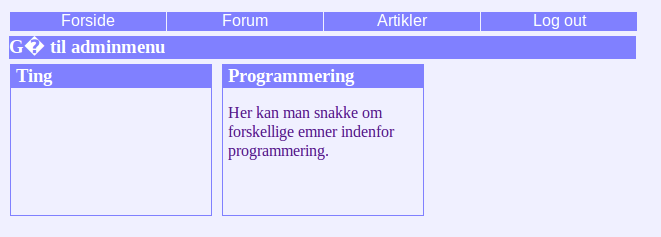
\includegraphics[width=100mm]{mi06.png}

Forum-forsiden findes ved at klikke på knappen 'Forum' i navigationsbaren. Her ses en oversigt over alle de kategorier der findes i forummet. Hver kategori vises som en boks med en overskrift (titlen på kategorien) og en beskrivelse. Hver boks er et link til en side der viser den pågældende kategori.

Hvis man er logget ind som en bruger med admin-rettigheder, vises der, ovenfor kategorierne, en knap med teksten 'Gå til admin menu'. Den linker til adminmenuen, hvor man kan redigere i kategorier og fora.

Forum-forsiden bruger et simpelt SQL udtræk fra kategori-databasen, som den sorterer efter categoryID så de nyeste kategorier vises først. Den tjekker om man er logget ind som administrator ved at hente isAdmin-feltet fra databasen for den bruger hvis ID svarer til det ID der er gemt i $\$$$\_$SESSION['LoggedIn'], og se om det er 1. I kode:

\lstinputlisting{MIForumCode/ex04.php}

Vi skriver et @ foran sessions-variablen for at fortælle PHP at den ikke skal sende warnings hvis variablen ikke findes. Den pæne måde at gøre det på er at tjekke om variablen er sat først, men det her har samme effekt.

\subsubsection[Adminmenuen]{Adminmenuen - adminmenu.php}
Her kan man redigere, oprette og slette fora og kategorier. Selve admin-menuens forside viser en liste af alle kategorierne, og et link med teksten 'Opret kategori', som fører til 'Opret kategori'-siden. Ud for hver kategori er der en slet-knap. Klikker man på slet-knappen, popper der en lille boks op og spørger om man er sikker på at man vil slette en hel kategori. Klikker man OK bliver kategorien og alle tilhørende fora, tråde og posts slettet. Klikker man på en kategori kommer man til 'Rediger kategori'-siden. 

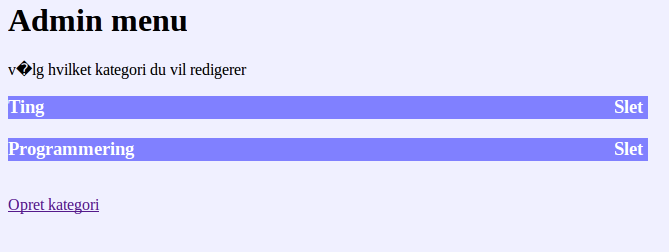
\includegraphics[width=100mm]{mi01.png}

Siden fungerer nogenlunde som forum-forsiden - i stedet for at lave pæne bokse, bliver hver kategori vist som et h3 element med en slet-knap til højre. Sletknappen er ikke et link, men kalder i stedet en JavaScript funktion som tager et ID som parameter. Funktionen laver et pop-up vindue som spørger om man er sikker på at man vil slette, og hvis man klikker OK, bliver window.location.href sat til den PHP-side der sørger for at slette kategorien.

\lstinputlisting{MIForumCode/ex05.htm}

\subsubsection[Rediger kategori og -forum siderne]{Rediger kategori og -forum siderne \\redcat.php, redigerforum.php, redcatquery.php, redforaquery.php}
Disse to sider er ret så ens - rediger kategori-siden giver mulighed for at ændre en kategori's navn og beskrivelse, samt oprette, redigere og slette fora der tilhører denne kategori. Rediger forum-siden giver mulighed for at redigere navn og beskrivelse for fora.

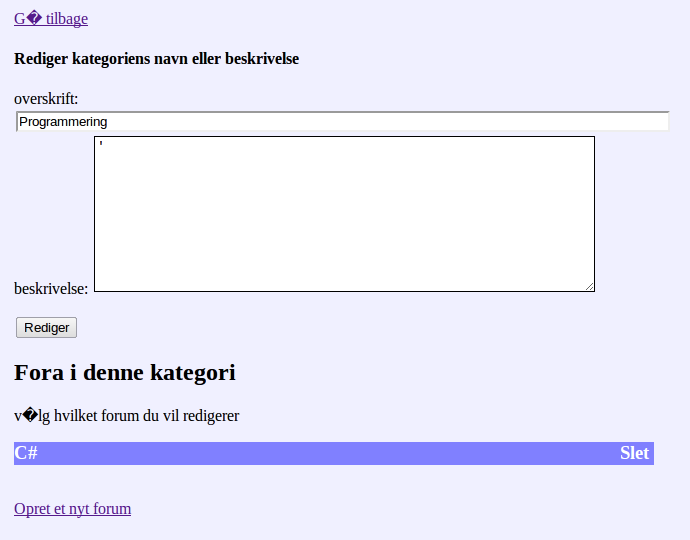
\includegraphics[width=100mm]{mi02.png}

Disse sider bruger samme tekstredigering og næsten samme SQL som siderne for at oprette kategorier og fora. Forskellen er at vi her trækker det gamle indhold ud af databasen først, og skriver det i tekst-boksene.

\subsubsection[Vis kategori]{Vis kategori - visfora.php}
Når man, på forum-forsiden, klikker på en kategori, kommer man til en side der viser en oversigt over alle fora i den pågældende kategori. 

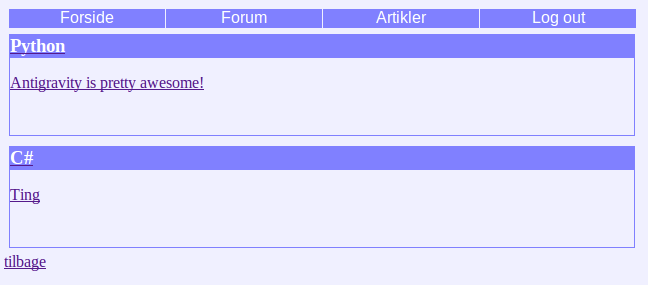
\includegraphics[width=100mm]{mi11.png}

Det er den samme PHP-fil der viser alle kategorier, den finder så de rette fora ud fra kategoriens ID, som sendes via $\$\_$GET-array'et. Vi bruger et SQL-udtræk til at hente alle fora hvor kategori-ID'et matcher, og viser dem med de nyeste først, på præcis samme måde som med kategorierne på forum-forsiden.

\subsubsection[Vis fora]{Vis fora - vistraade.php}
Foraer bliver vist meget på samme måde som kategorier - en liste af alle tråde i det pågældende fora, sorteret med de nyeste først. Forskellen er at brugere her har muligheden for at oprette tråde.

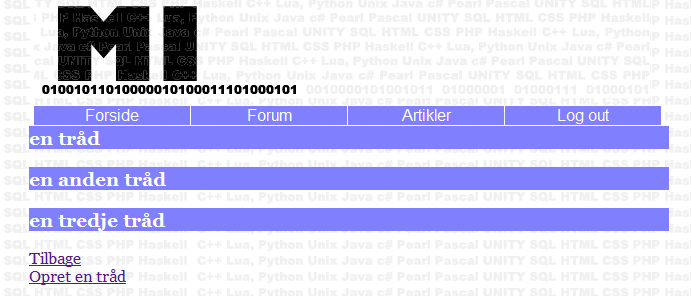
\includegraphics[width=100mm]{mi16.png}

\subsubsection[Vis tråd]{Vis tråd - viewThread.php}
Når man, på Vis Fora siden, klikker på en af de viste tråde, kommer man til denne side. Her vises først titlen og den tekst tråd-staren skrev, derefter alle de posts der er skrevet i tråden. Ved hver post vises navnet på den bruger der har skrevet den.

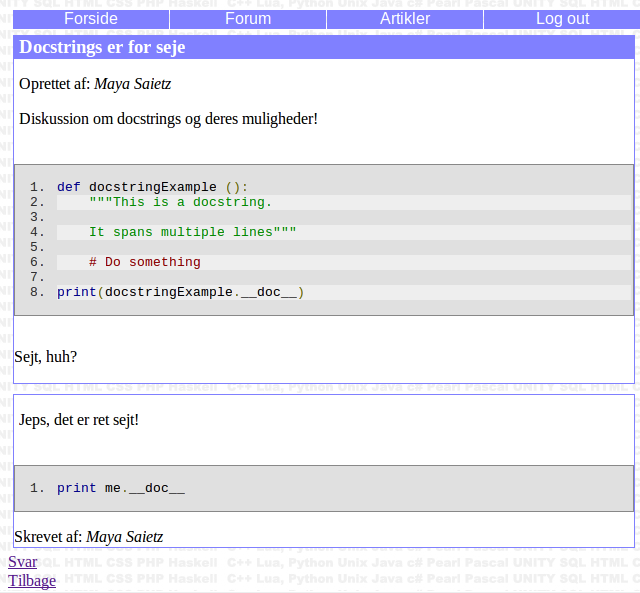
\includegraphics[width=100mm]{mi12.png}

Nederst på siden vises der en Tilbage-knap som fører til Vis Fora siden, og, hvis man er logget ind, en Svar-knap.

Siden fungerer ved hjælp af to queries - et der finder åbningsposten i threads-tabellen, og et der finder de resterende posts i post-tabellen. Posts vises vha. et while-loop, som udskriver en bunke javascript der sørger for at formatere teksten rigtigt.

\subsubsection[Opret tråd]{Opret tråd - oprettraad.php, ny-traad.php}

Denne side kommer man til ved at klikke på linket 'Opret tråd' på Vis fora-siden. Her kan man skrive et nyt emne på forummet. Det foregår ved hjælp af samme JavaScript text editor som til artikel-siden.

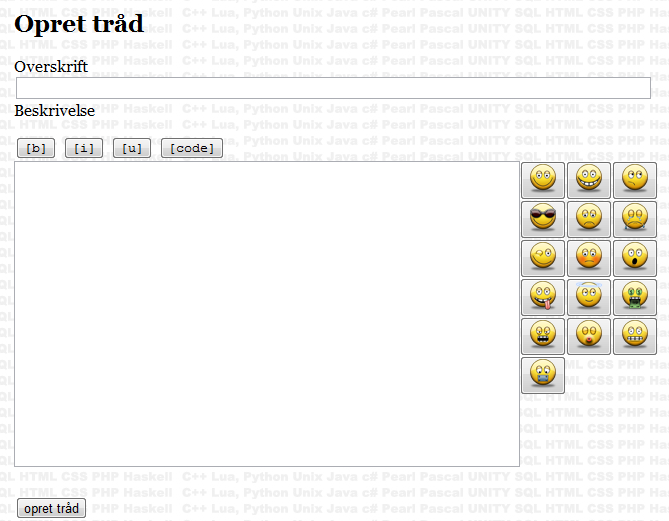
\includegraphics[width=100mm]{mi17.png}

Text editoren kan bl.a. lave [code][/code] tags, som resulterer i at den tekst der står imellem vil blive stillet op med en monospace font og farvelagt alt efter hvilket sprog det er. Det gør det nemt at bruge forummet til at diskutere programmerings-problemer ved simpelthen at skrive den problematiske kode på denne måde.

\subsubsection[Svar på tråd]{Svar på tråd - writePost.php, createPost.php}

Denne side virker præcis som Opret tråd-siden, med den undtagelse at man ikke kan skrive en titel. Den bruges til at besvare tråde, og hvad der skrives her havner i post-tabellen i vores database, hvor det kan identificeres ved trådens ID.

\subsubsection[Artikel-forsiden]{Artikel-forsiden - articles.php}
Når man klikker på knappen 'Artikler' i navigations-baren kommer man til denne side. Her er alle artikler listet ved navn, og man kan klikke på dem for at læse artiklen. Nederst på siden er der et link - hvis man er logget ind står der 'Skriv ny artikel', og det fører til en side hvor man kan - hold fast - skrive en ny artikel! Hvis ikke man er logget ind, står der 'Log ind for at skrive en ny artikel', og linket fører til login-siden.

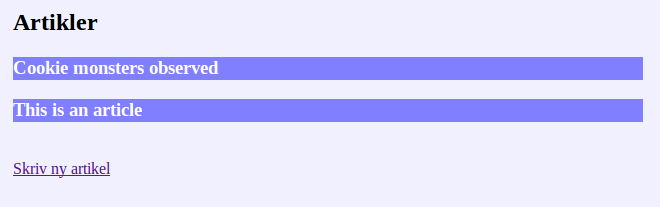
\includegraphics[width=100mm]{mi05.png}

Siden fungerer med et SQL query der henter alle artikler fra databasen og viser dem som h3 elementer.

\lstinputlisting{MIForumCode/ex01.php}

\subsubsection[Vis artikel]{Vis artikel - viewArticle.php}
Dette er den side man bliver taget til når man klikker på en artikel på Artikel-forsiden. Her vises den pågældende artikel med titel og forfatter efterfulgt af hele teksten. Hvis man er logget ind som den bruger der har oprettet artiklen, kan man redigere eller slette den ved hjælp af to links i bunden af siden.

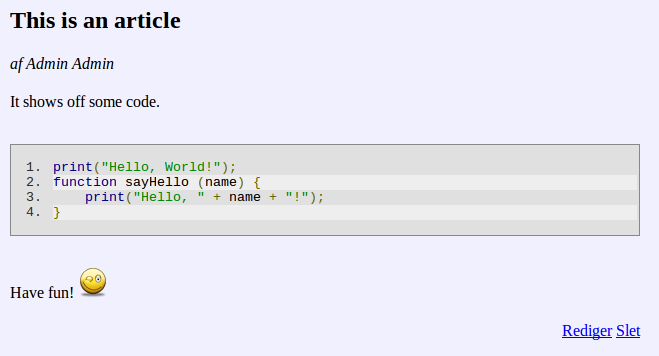
\includegraphics[width=100mm]{mi10.png}

Siden fungerer ved at kigge i databasen efter en artikel med det ID som er angivet i GET-array'et. Hvis en sådan ikke findes, bliver man sendt tilbage til artikel-forsiden. Ellers bliver artiklen vist. Desuden sammenlignes artiklens writerID med den nuværende brugers ID, og hvis de er ens (eller hvis brugeren er administrator) vises links for at redigere og slette artiklen. Her er et par af de mere interessante ting fra koden:

\lstinputlisting{MIForumCode/ex02.php}

Dette script involverer, som kan ses i ovenstående kode-listing, et grimt hack hvor PHP udskriver JavaScript. Det er nødvendigt for at kunne behandle vores hjemmelavede bbcodes og formatere koden pænt.

\subsubsection[Skriv artikel]{Skriv artikel - writeArticle.php, createArticle.php}
Denne side giver mulighed for at skrive nye artikler til siden. De bliver så vist under artikel-sektionend forside, og på forsiden når de er nye. Den fungerer ved hjælp af en text-editor skrevet i JavaScript. Dette giver mulighed for at bruge nogle hjemmelaved bbcodes, enten ved at indtaste dem eller ved at trykke på knapperne som findes ovenfor og til højre for textboksen.

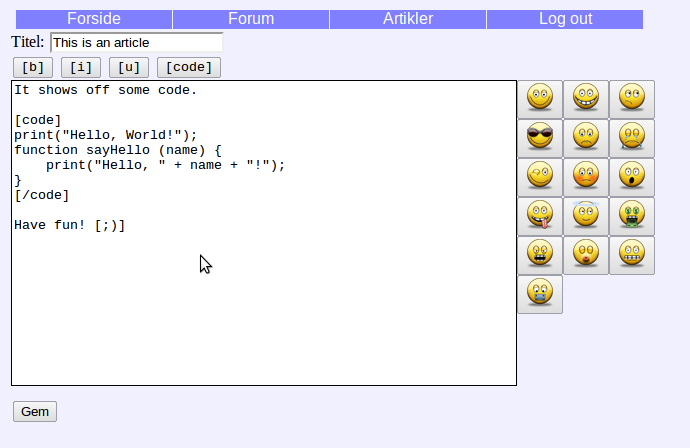
\includegraphics[width=100mm]{mi04.png}

Selve det JavaScript det sørger for at text-editoren virker er for langt til at inkludere her, men kan ses i text$\_$edit.js. Et uddrag der dog er interessant at kigge på er funktionen for at sætte tags rundt om et markeret stykke tekst:

\lstinputlisting{MIForumCode/ex03.js}

Den deler teksten i tre dele, sætter de angivne tags ind og sætter det hele sammen til en lang string igen. Bemærk den IE-specifikke kode - IE har ikke nogen funktion for at finde start og slut på en markering, så man er nød til at beregne placeringen ud fra længen af den markerede tekst, og så sætte de to variable manuelt. Derefter kan man fortsætte som normalt.

\subsubsection[Rediger artikel]{Rediger artikel - editArticle.php, deleteArticle.php}
Denne side fungerer mere eller mindre som Skriv artikel, med den undtagelse af at den henter den gamle tekst og titel fra databasen først, og at den bruger UPDATE frem for INSERT INTO. Desuden er den kun tilgængelig hvis man er logget ind som den bruger der har skrevet artiklen eller en admin.

\subsubsection[Login-siden]{Login-siden - login.php, loginBackend.php}
Dette er stedet hvor man logger ind som bruger. Man kan komme herhen ved at klikke på knappen 'Log ind' i navigationsbaren, eller via et af de mange links som findes på steder hvor vi regner med at det er nyttigt at logge ind, så som artikel-forsiden hvor man kan logge ind for at skrive en ny artikel.

\begin{center}
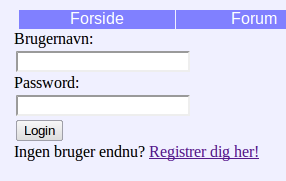
\includegraphics[width=50mm]{mi07.png}
\end{center}

Siden består af en standard login form, hvor brugeren kan indtaste sit navn og løsen, og en knap med teksten 'Login'. Når man trykker på knappen, bliver indtastningerne tjekket i forhold til databasen, og hvis de passer, bliver man logget ind. Hvis man ikke har en bruger er der et link til registreringssiden lige under login-formen.

Hvis man indtaster en kombination af brugernavn og løsen som ikke findes i databasen, vises fejlmeddelsen 'Forkert brugernavn eller adgangskode' i rød tekst. Hvis man mangler at udfylde et af felterne, vises fejlmeddelelsen 'Manglende brugernavn eller adgangskode' i rød tekst. 

\begin{center}
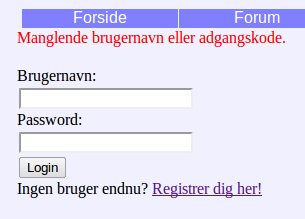
\includegraphics[width=50mm]{mi09.png}
\end{center}

Login-formen er en ganske almindelig html form, hvis submit-knap sender os til et backend-script som så tager sig af SQL-koden. Til at tjekke om brugere findes, bruger vi følgende SQL query:

\lstinputlisting{MIForumCode/ex08.php}

Bemærk at vi kører md5 \emph{efter} at have kørt mysql$\_$real$\_$escape$\_$string() - rækkefølgen skal være den samme som på registreringssiden. Egentlig er det ikke nødvendigt at escape løsenet, da det ikke kan gøre nogen skade i krypteret form, men det er en god vane aldrig at putte ting i queries uden at have kørt dem igennem en escape-funktion.

Hvis man logges ind successfuldt, redirectes man til index-siden. Ellers bliver man sendt tilbage til login-siden med en fejlkode - denne metode vil blive beskrevet nærmere under afsnittet om registreringssiden.

\subsubsection[Registrerinssiden]{Registreringssiden - register.php, registerBackend.php}
Her kan nye brugere registrere sig. Dette foregår ved at udfylde en række felter med ting som brugernavn, løsen, email, navn m.v. Der er desuden en knap med teksten 'Registrer', hvor brugeren kan klikke når hun har udfyldt alle felter.

\begin{center}
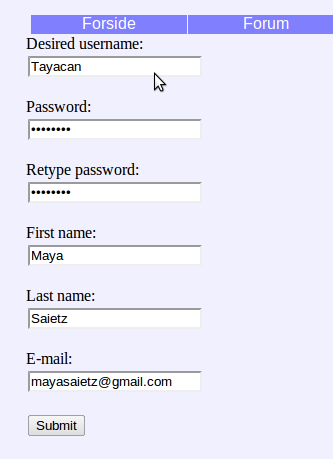
\includegraphics[width=50mm]{mi08.png}
\end{center}

Hvis der er felter som ikke er udfyldt, vises fejlmeddelelsen 'Venligst udfyld alle felter'.

Siden består af en html form som håndterer brugerinput og en stump PHP-kode som håndterer fejlmeddelelser. Vi benytter os af den form for fejlhåndtering mange steder i koden, så her er et eksempel:

\lstinputlisting{MIForumCode/ex06.php}

Som man kan se på koden bruger vi GET-array'et til at sende vores fejlmeddelelser.

Submit-knappen på registreringssiden leder til vores backend script, som sørger for at tjekke at input er gyldigt, krypterer koden, og kører de relevante SQL queries. Desuden sørger det for at sanitere alt brugerinput med mysql$\_$real$\_$escape$\_$string(). 

Hvis input nu \emph{ikke} er gyldigt, sender scriptet os tilbage til registreringssiden med en fejlkode, sådan her:

\lstinputlisting{MIForumCode/ex07.php}

\subsection{Andre scripts}
De følgende scripts har været af betydning for hele siden, men er ikke noget brugeren lægger mærke til.

\subsubsection{util.php}
Dette script indeholder en række funktioner som frit kan bruges overalt på siden. For eksempel bruges funktionerne top() og bottom() på alle sider, til at lave menuen, headeren, og bottom() til at afslutte tags. Alt synligt indhold skal placeres mellem kald til disse to funktioner.

\subsubsection{config.php og install.php}
Disse to scripts tager sig af at oprette og konfiguerere databasen. Man åbner install.php i sin browser, indtaster sit brugernavn og password til MySQL, og så opretter config.php automatisk en database samt en bruger som har fuld rettighed til at ændre i den, men kun den, database. På den måde sikres det at selv hvis siden skulle blive hacket, går det kun ud over den ene database.

\subsubsection{auth.php}
Dette script skal require's på alle sider som kræver at man er logget ind. Hvis en bruger som ikke er logget ind navigerer til en side hvor auth.php er med, vil browseren automatisk blive redirectet til login-formen.

\subsubsection{logout.php}
Dette er et script som log ud-knappen linker til. Det sørger for at slette alle sessionsvariable, og forsøger derefter at sende en til den side hvor man var da man loggede ud.

\subsubsection{connect.php}
Dette script står for at forbinde til databasen. Alle sider som skal have med databasen at gøre, behøver kun at include dette script for at have forbindelse.

\section{Afprøvning af siden}
Vi har under arbejdet med siden afprøvet den konstant. Jo mere man laver mellem hver afprøvning, jo sværere er fejlene at finde, så hvis vi kan lave en lille ting og sikre os at det virker, og så bruge den lille ting til at bygge noget større, er det bedst. For eksempel starter man måske med at sikre at man får fat i de rigtige værdier fra sin database ved bare at printe dem ud, inden man begynder at vise dem pænt - på den måde ved man at det er visningen der er gået galt hvis der pludselig ikke dukker noget op på skærmen.

Vi har eksperimenteret med alle former for manglende og korrupt input vi kunne komme i tanke om, bl.a. html tags, PHP kode og SQL injections, og mener efterhånden at have sikret vores side mod alle angreb fra den front. Ud over det bruger vi $\$$$\_$POST frem for \$\_REQUEST når vi skal bruge variable fra POST-array'et, så brugere ikke kan taste interessante ting i URL'en.

\subsection{Typiske problemer}
Dette er listen over de problemer vi blev ved med at løbe ind i gennem arbejdet med siden. De kunne være nyttige at huske på til fremtidige projekter.

\begin{itemize}
	\item At skrive POST med småt. \\
		$\$$$\_$post er ikke det samme.
	\item At glemme underscore foran post. \\
		$\$$POST virker heller ikke.
	\item At glemme at sende værdier med GET-array'et. \\
		Vi har haft masser af 'undefined index'-fejl.
	\item At glemme at køre sit SQL query. \\
		mysql$\_$query()! For helvede!
	\item At glemme at rette variabelnavne i copy-pastet kode. \\
		Jamen det virkede på den anden side!
\end{itemize}

\end{document}
